\chapter{Introduction}
\label{chapter:Introduction}
\section{Coreference resolution}

Coreference resolution is the process of determining whether two or more expressions in natural language refer to same entity in the real world [4]. Coreference resolution is an important and challenging task of natural language processing (NLP) [1][5]. It is believed to be useful in question answering, information extraction, relationship extraction and document summarization among others. \vspace{5mm}
  
\emph{Example (1):}
\begin{changemargin}{10mm}{10mm} 
   \emph{ M-CSF treatment was also associated with a rapid induction of \textbf{the jun-B gene}, although expression of \textbf{this gene} was prolonged compared to that of c-jun.}          
   \vspace{5mm} 
\end{changemargin} 

In example (1), \emph{\textbf{ "the jun-B gene"}} and \emph{ \textbf{"this gene"}} refer to same entity in the real world. Therefore, we can say that these two expressions corefer. Another characteristic of these two expressions is that the second expression is semantically dependent on the first.

This dependency of corefering expressions leads to a new linguistic phenomenon called anaphora. Linguists have given various different definitions for these two linguistic terms, which leads to a conflusion between coreference and anaphora. Sometimes researchers do not distinguish these two terms and say that they are synonyms [2]. For clarification, in the following paragraphs I will give the definitions of anaphora and coreference that we will use throughout the thesis.
  
Anaphora (anaphoric expression) is the linguistic phenomenon of pointing back to a previously mentioned expression in the text. The expression mentioned in the text which an anaphora points to is called the antecedent. Anaphora resolution is the process of finding the antecedent of an anaphoric expression [73]. In other words, it means finding pairs of anaphoras and antecedents. As illustration, in example (1) \emph{\textbf{ "the jun-B gene"}} is an anaphoric expression (anaphora) because it refers back to its antecedent, \emph{ \textbf{"this gene"}}. 

If the antecedent and anaphora refer to a same entity in the real world they are coreferential [73].

Gasperin defines anaphora as a directed relation between two linguistic expressions in the text, where the reader, in order to interpret the second expression, is referred back to the first one. In Figure 1.1 we can see the intersection and difference between coreference and anaphora. The intersection of these two terms is coreferent anaphora. Thus, a coreferent anaphora is when the anaphora is dependent from the antecedent and they refer to same entity.[49]

Associative anaphora is a relation between two expressions where the anaphora's interpretation depends on the antecedent, but nevertheless, they do not semantically refer to a same entity. In example 2, \emph{"the door"} is an associative anaphora and its antecedent is \emph{"the room"}, because to interpret the expression\emph{"the door"} we need to refer back to the expression \emph{"the room"}.\\

\emph{Example (2):}
\begin{changemargin}{10mm}{10mm} 
   \emph{  The student entered in \textbf{the room}. He did not close \textbf{ the door}.}
   \vspace{5mm} 
\end{changemargin}  
\begin{figure}[ht]
   \begin{center}
	  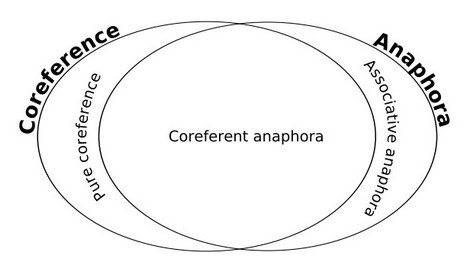
\includegraphics[scale=1.]{corefVsAnaphora.jpg} 
 	  \caption[Difference between anaphora and coreference]{Difference between anaphora and coreference [49]}
	  \label{Figure 1}
   \end{center}
\end{figure}

Kees van Deemter and Kibble [24] define coreference relation of two expressions as the logical equivalence relation where both expressions \emph{"refer to the same entity"}.
 
Mathematically, defining Referent$(\alpha_1)$ as the\emph{"the entity referred to by $\alpha_1$"}, a coreference relation for expressions $\alpha_1$ and $\alpha_2$ holds if and only if 
\begin{center}
  Referent $(\alpha_1)$ = Referent $(\alpha_2)$
\end{center}
 
Hence, coreference is an equivalence relation (reflexive, symmetric and transitive relations). From symmetric relation, the conclusion is that $\alpha_1$ and $\alpha_2$ are semantically independent. Furthermore, the authors [24] define anaphoric relation of two expressions $\alpha_1$ (antecedent) and $\alpha_2$ (anaphora), if and only if $\alpha_2$ depends on $\alpha_1$ for its interpretation. 
 
Summarizing, anaphora resolution is the task of finding mentions (anaphoras) that are dependent in their interpretation on a second expression (their antecedent). On the other hand, coreference resolution can be seen as a clustering task, where we must find all mentions in the text that refer to same entity.

\section{Coreference resolution in Biomedical literature}

In biomedical literature, there exists just one corpus that deals with coreference resolution. This corpus was published by the BioNLP group. In it, the community defined the task named Protein Coreference Resolution. I will describe in the following sections the detailed specification of this task.

\subsection{Data description}

The BioNLP corpus consists of 1210 annotated abstracts. The corpus is divided into 3 subsets: 800 abstracts in the training set, 150 in the development set, and 250 in the test set. Each document is annotated with proteins, anaphoric expressions and their references. For each abstract, three files exist:
\begin{itemize}
  \item A text file, which contains the content of the abstract.
  \item A protein annotation file, which contains the annotated proteins.
  \item A relation file, which contains the coreference relation.
\end{itemize}

\newpage
\begin{figure}[ht]
   \begin{center}
	  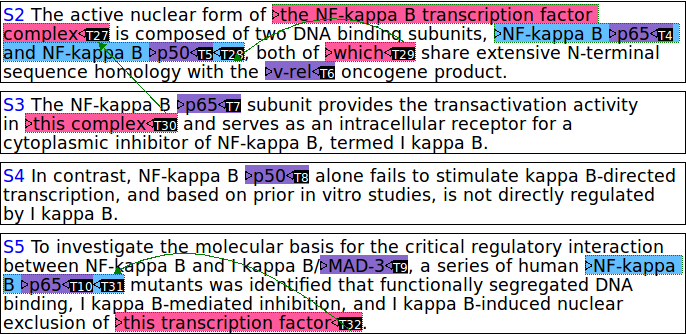
\includegraphics[scale=0.6]{bioNLP.jpg} 
      \caption[Example of file annotation]{Example of file annotation\footnotemark}
	  \label{Figure 2}
   \end{center}
\end{figure}
\footnotetext{Figure taken from [63]}

I will clarify the content of the protein annotation and coreference relation files by examples. In Figure 1 annotations T4-10, marked with purple color, are protein annotations. Every protein name mentioned in the text is annotated. Each annotation consist of its id, offsets (begin span and end span) and its string content, and this information is inserted in the protein annotation file as in Example (3).\\

\emph{Example (3):}
{\fontfamily{qcr}\selectfont
	\begin{tabbing}
		\hspace{3cm} T4	\hspace{5mm}\=  Protein 275 278	\hspace{5mm} \= p65\\
		\hspace{3cm} T5 \> Protein 294 297 \> p50\\
		\hspace{3cm} T6	\> Protein 367 372 \> v-rel\\
		\hspace{3cm} T7	\> Protein 406 409 \> p65\\
		\hspace{3cm} T8	\> Protein 597 600 \> p50\\
		\hspace{3cm} T9	\> Protein 843 848 \> MAD-3\\
		\hspace{3cm} T10 \> Protein 879 882 \> p65\\
	\end{tabbing}
}
\vspace{5mm} 

\emph{In Example (3), the first line indicates that in the text there is a protein reference \textbf{"p65"} that begins at 275th character and its content ends before 278th character. This annotation is indexed by the id, "T4" [1].}

The coreference relation file contains three types of annotations: anaphoric annotations, their antecedent, and coreference relations. In Example (4), annotations T27-32 are of the first and second type and the R1-R3 describe coreference relation of expressions. Most of the anaphoric expressions are: pronouns (relative, personal, possessive, reflexive) and definite nouns (e.g. this protein).\\

\emph{Example (4)\footnotemark :}
{\fontfamily{qcr}\selectfont
	\begin{tabbing}
		T27 \= Exp 179 222\hspace{3mm} \= the NF-kappa B TF compl 215 222 compl \\
		T28 \> Exp 264 297 \> NF-kappa B p65 and NF-kappa B p50\\
		T29 \> Exp 307 312 \> which\\
		T30 \> Exp 459 471 \> this complex \hspace{2mm}   464 471 complex \\
		T31 \> Exp 868 882 \> NF-kappa B p65\\
		T32 \> Exp 1022 1047 \> this TF   1027 1047  trans. factor\\
		R1  \hspace{5mm} \=  Coref Anaphora:T29 Antecedent:T28  \hspace{5mm}  \= [T5, T4]\\
		R2 \>  Coref Anaphora:T30 Antecedent:T27\\
		R3 \>  Coref Anaphora:T32 Antecedent:T31  \>  [T10]\\
	\end{tabbing}
}
\footnotetext{Transcription factor is shorten in TF and complex in compl because of limited line space}
\vspace{5mm} 

\emph{In Example (4), the first line indicates that in the offset 179-222 of the abstract there is a protein mention "the NF-kappa B transcription factor complex". Its minimal , which still carries its meaning, is "complex" (215-222), and this annotation has the index "T27". In this way, every annotation (a protein mention or an expression that refers to a protein) is described in the coreference relation file.}

\emph{The last line describes the coreference relation between mentions T32 and T31. Also, we can see that mention T32 is an anaphora and refers to T31, which in its string contains a protein name T10 (p65). So, here we see that we have two types of coreference relations. The first type of relation is between two corefering mentions, like T32 with T31, and the second type of relation is between a mention and a protein name (T32 with T10).}

\subsection{Task description and evaluation}

For both types of coreference relations the BioNLP community (mentioned in the previous section) defined a sub-task. First relation type is named surface coreference resolution and the latter is named protein coreference resolution.

For both tasks, the resolver receives a text and a protein annotation file, and as output should return all protein mentions with their offsets and coreference relations between mentions. The result should be a file similar to Example (3), with all detected protein mentions and relations. 

\subsection{Evaluation Measures}

In this section, I will define the Protein Coreference Resolution task(in abstracts and full text) mathematically and its evaluation measures. The task($f$) of protein coreference resolution, which is defined by the BioNLP community, I define formally in the following way:" given a text (abstract) $T$ with annotated protein names $P$, the system should return ordered couples $(x, y)$ where $y$  is the antecedent of $x$".\\
\begin{center}
  $f(X,P)=\{(x_i,y_i) |i=1..n \And Antecedent(y_i)=x_i \And y_i= protein$  $name\}$ \\
  $X-string$ \\
\end{center}

$P$ is a set of ordered set defined in the following way:\\
\begin{center}
    $P= \{(start_j, end_j, protein_j)| j=1..n \And start_j< end_j \And |protein_j|= end_j-start_j\}$\\
\end{center}
 
The system that I built produce three types of anaphora-antecedent links(pairs):

\begin{itemize}
  \item correct response links
  \item missing links
  \item spurious response links.
\end{itemize}
From these three types of links we can derive:
\begin{itemize}	
 \item $true$ $positive$ $(tp)$ - number of  correct anaphora-antecedent links - links that the system correctly predicted\\
 \item $true$ $negative$ $(tn)$ - number of missing anaphora-antecedent links - links that the system did not find\\
 \item $false$ $positive$ $(fp)$ - number of spurious anaphora-antecedent links - links that the system predicted wrong \\
\end{itemize}
To measure the accuracy of the system we use the traditional  precision, recall and F-score  measurement which are defined in the following way\\
\hspace{2cm}  Precision: \hspace{1cm}\\
\hspace{4cm}\[ \scalebox{1.2} {$P =\frac{tp}{tp+fp}$}\] \\
\hspace{2cm} Recall: \\
\hspace{4cm} \[ \scalebox{1.2} {$R=\frac{tp}{tp+tn}$}\] \\
F-score is taken as equally weighted harmonic mean of precision and recall:\\
\[ \scalebox{1.2} {$F(\beta)=(1+\beta^2)\cdot \frac{P\cdot R}{\beta^2P+R}$}\] \\
 and for $\beta=1$ \\
\[ \scalebox{1.2} {$F(1)=2\cdot \frac{P \cdot R}{P+R}$}\]\\
\subsection{Evaluation measures in BioNLP Protein coreference resolution}

In the surface coreference mode, the resolvers should find anaphoric protein expressions and their antecedents, regardless of whether antecedent actually embed protein names or not. 
The protein coreference mode evaluates the performance of finding anaphoric protein references, which their antecedent contains a protein name. 
My main focus in this thesis was to build a system which achieves high accuracy in protein coreference mode. Thus, I will describe the scoring principle of protein coreference mode using an example.

From example (4) we take relation \emph{"R1 Coref Anaphora:T29 Antecedent:T28 [T5, T4]"}. Antecedent T28 contains two protein names \emph{p50} and \emph{p65}. So, in the protein coreference mode, we check whether (T29, T5) and (T29,T4) are predicted or not. For each of these pairs, if the system predicted, it gets 1 point. The whole R1 has two points. If the system finds just (T29,T5), it gets 1 point. Wrong predicted pairs decrease the system's precision. 

\subsection{Importance of coreference resolution}

Why is coreference task important in biomedical domain?

Coreference resolution is believed to be useful for improved event and relationship extraction [2]. Until now we do not have concrete results to prove that the coreference resolution improves the Information extraction in biomedical domain, because the protein coreference task did not have enough good results and the motivation of this thesis was to build a high accurate coreference resolution system.
 
In other domains, anaphora resolution improves results in different information extraction and machine translation tasks (see section 2), but still the improvements are not as expected because of the accuracy of current anaphora resolution systems[9,10,11,12].
 
Anaphora resolution is not a high-accuracy task for information extraction (IE) systems but properly resolving some kinds of coreference is usually difficult even for humans annotators, who achieved about 80 percent [8].


